% Source of Capmcm24201771_paper_en_extended.pdf. Build in this folder with two runs of
%   xelatex -jobname=Capmcm24201771_paper_en_extended main.tex
% (fonts: TeX Gyre Termes/Heros, STIX Two Math, Noto Serif CJK SC) and copy Capmcm24201771_paper_en_extended.pdf to ../
\documentclass[a4paper,11pt]{article}
\usepackage{fontspec}
\setmainfont{TeX Gyre Termes}
\setsansfont{TeX Gyre Heros}
\newfontfamily\cjkfont{Noto Serif CJK SC}
\usepackage{amsmath}
\usepackage{unicode-math}
\setmathfont{STIXTwoMath-Regular.otf}
\usepackage[a4paper,top=2.5cm,bottom=2.4cm,left=2.6cm,right=2.6cm]{geometry}
\usepackage{graphicx,booktabs,array,threeparttable,pdfpages,fancyhdr,xurl}
\usepackage[font=small,labelsep=period,skip=4pt]{caption}
\usepackage[hidelinks,bookmarksnumbered=true,bookmarksopen=true]{hyperref}
\usepackage{titlesec}
\renewcommand{\floatpagefraction}{0.8}\renewcommand{\topfraction}{0.88}\renewcommand{\bottomfraction}{0.7}\renewcommand{\textfraction}{0.1}
\usepackage{etoolbox}\AtBeginEnvironment{thebibliography}{\small\linespread{1.05}\selectfont\setlength{\itemsep}{1pt}\setlength{\parskip}{0pt}}
\setlength{\emergencystretch}{3em}
\linespread{1.15}
\setlength{\parskip}{0.25em}
\titleformat{\section}{\large\bfseries}{E\arabic{section}}{0.8em}{}
\titleformat{\subsection}{\normalsize\bfseries}{E\arabic{section}.\arabic{subsection}}{0.6em}{}
\renewcommand{\thesection}{E\arabic{section}}
\renewcommand{\thefigure}{E\arabic{figure}}
\renewcommand{\thetable}{E\arabic{table}}
\renewcommand{\theequation}{E\arabic{equation}}
\setlength{\headheight}{15pt}\pagestyle{fancy}\fancyhf{}\renewcommand{\headrulewidth}{0.4pt}
\newcommand{\hd}[1]{\begin{tabular}[b]{@{}c@{}}#1\end{tabular}}
\newcommand{\exthead}[1]{\fancyhead[L]{\small #1}\fancyhead[R]{\small Part II\quad Post-competition extensions}\fancyfoot[C]{\small E-\thepage}}

\graphicspath{{../../figures/extension/}}
\hypersetup{pdftitle={China's pet industry: forecasts, demand, coupling and policy impact -- extended edition}}
\begin{document}
\thispagestyle{empty}
\begin{center}
{\Large\bfseries China's Pet Industry: Population Forecasts, Global Demand,\\[0.2em] Industry Coupling and Policy Impact}\\[0.7em]
{\large Extended edition --- note}
\end{center}
\vspace{0.8em}

This file has two parts. Part I is the paper submitted to Problem C of the 2024 APMCM Asia-Pacific Mathematical Contest in Modeling (32 pages), reproduced exactly as submitted. Part II, starting on page E-1, contains post-competition extensions written in November 2026.

The paper forecasts China's urban cat and dog populations from five annual observations (2019--2023) with a combination of a linear trend, a grey model GM(1,1) and an ARIMA model, and builds on these forecasts for the demand, coupling and policy questions. Part II tests the forecasting layer, which is the only part whose inputs can be reconstructed. E1 compares the forecasts with the populations published afterwards: one year ahead the errors are within $\pm 3$\,\%, but the cat forecast is 7.3\,\% too high after two years and the dog forecast has the wrong sign of change. E2 asks whether this was bad luck or a property of the method, by evaluating the same method family on the 1\,088 annual demographic series of the M4 forecasting competition. The paper's linear trend is the least accurate trended method at every horizon, and its classical 95\,\% prediction intervals contain the outcome in only 72\,\% of cases three years ahead, against 93\,\% for intervals calibrated on the reference class.

A reading note on Part I: the summary sheet prints the 2026 cat forecast as ``8.386 million'' and the dog forecasts as ``5.06--5.1 million''. The underlying series are in units of $10^4$ animals, so the intended values are 83.86 million and 50.6--51 million.

Every number in Part II can be reproduced with the scripts in the \texttt{extension/} folder of the code repository; result files are in \texttt{results/extension/}. The M4 files are downloaded at run time and are not redistributed. The original code and data of the 2024 entry were not preserved.

\clearpage
\pdfbookmark[0]{Part I\quad Competition paper (as submitted)}{part1}
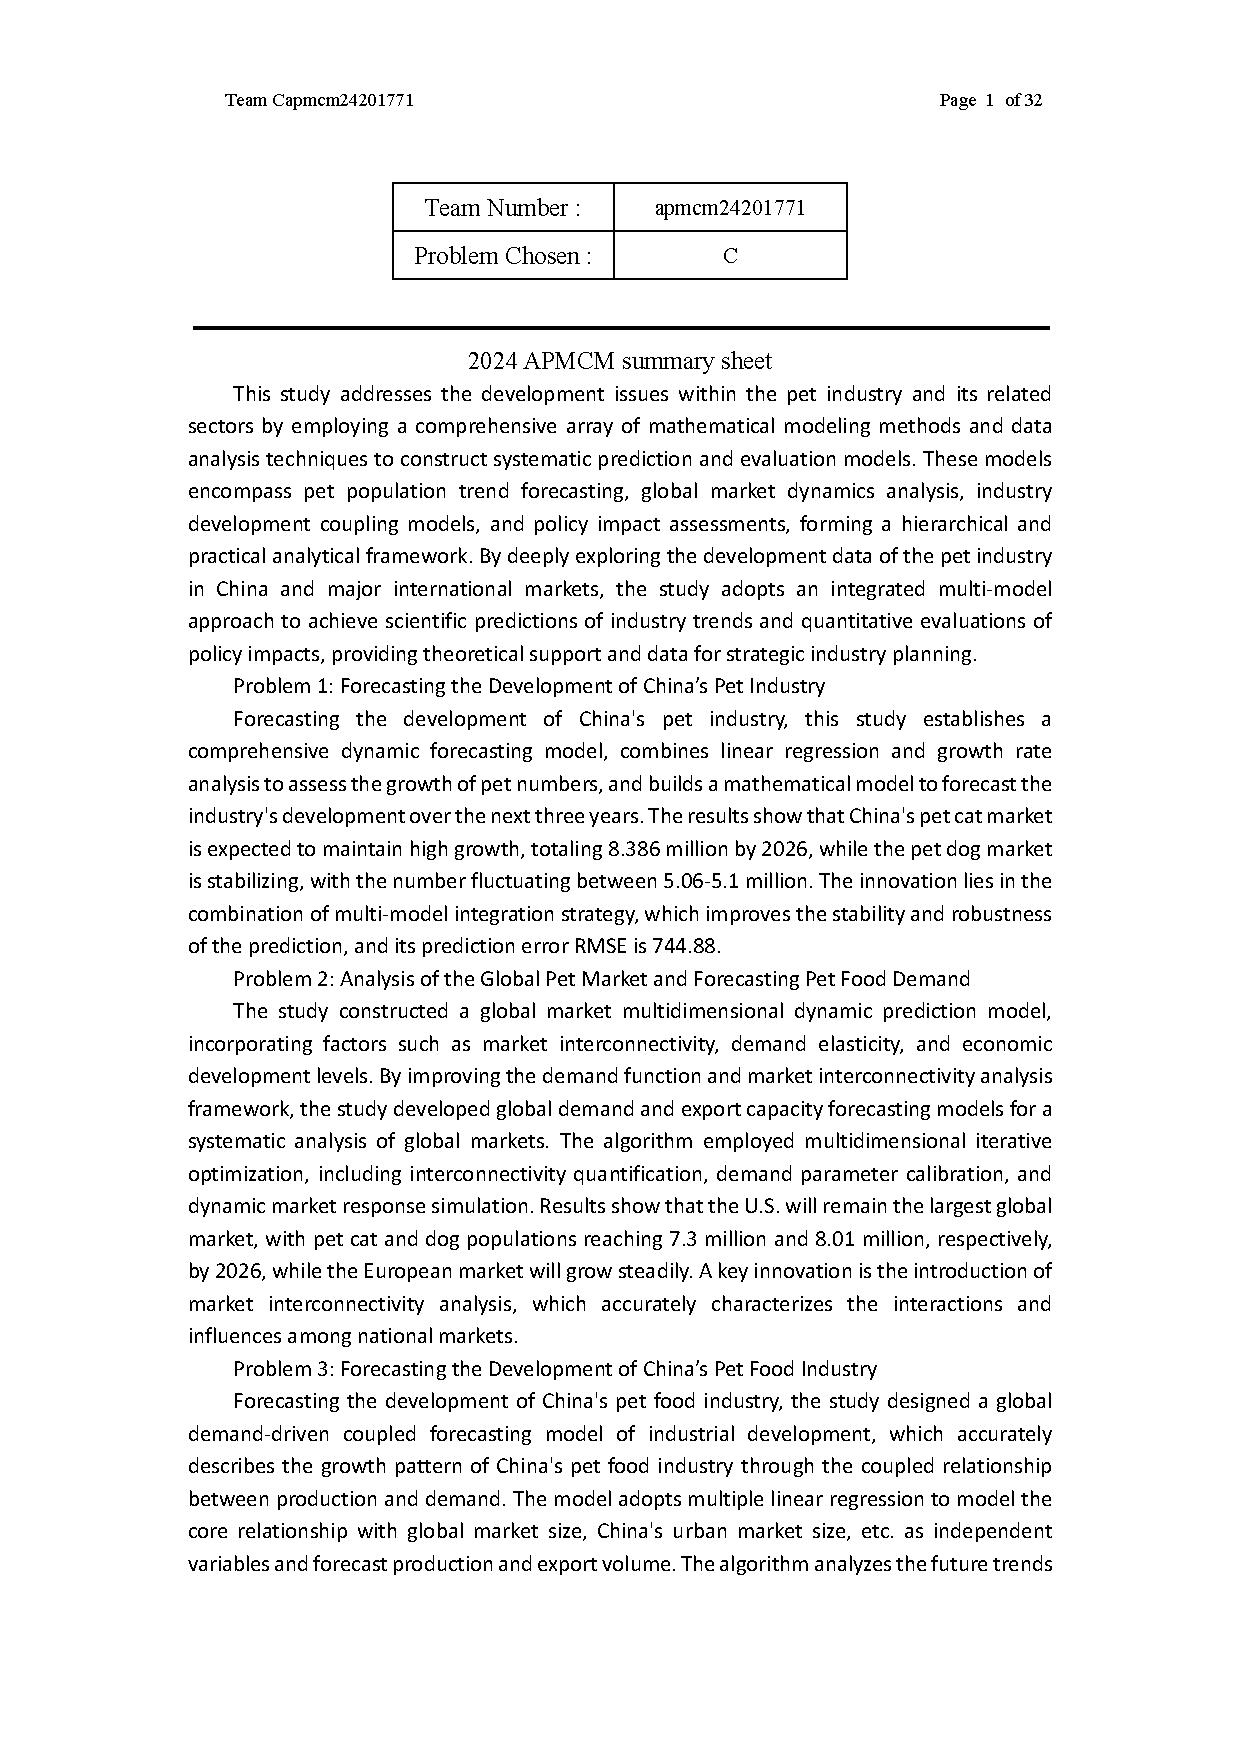
\includepdf[pages=-]{../Capmcm24201771_paper_en.pdf}
\pdfbookmark[0]{Part II\quad Post-competition extensions}{part2}
\setcounter{page}{1}
\exthead{China's pet industry}
\begin{center}{\Large\bfseries Part II\quad Post-competition extensions}\end{center}

Problem 1 of the paper forecasts the urban cat and dog populations of China for 2024--2026 from the five annual values of 2019--2023. The combined model puts cats at 72.97 million in 2024 and 83.86 million in 2026 (a compound growth rate of about 7.3\,\% a year) and keeps dogs nearly flat (51.1 million in 2024, 50.6 million in 2026). These forecasts feed the demand and industry models of Problems 2--4. Two years of new data have since been published, which makes the forecasting layer testable. E1 compares the forecasts with what was observed. E2 places that single comparison in a reference class of real series, which separates the behaviour of the method from the particular outcome of 2024--2025, and replaces the point forecasts with calibrated intervals.

\section{Forecasts versus what happened}

The China Pet Industry White Paper, the data source family used in the paper, published 2024 values in its 2025 edition and 2025 values in its 2026 edition\cite{petdata}. The paper reports forecasts for 2024 and 2026; the 2025 value is interpolated geometrically between them. Table~\ref{tab:pet-e1} compares forecasts and observations.

\begin{table}[htbp]\centering\small
\caption{The paper's Problem-1 forecasts against the populations published afterwards (urban China, $10^4$ animals). Growth is year on year.}\label{tab:pet-e1}
\begin{tabular}{lrrrrr}\toprule
Species, year & Forecast & Observed & Error & Forecast growth & Observed growth\\\midrule
Cats, 2024 & 7\,297 & 7\,153 & $+2.0$\,\% & $+4.5$\,\% & $+2.5$\,\%\\
Cats, 2025 & 7\,823 & 7\,289 & $+7.3$\,\% & $+7.2$\,\% & $+1.9$\,\%\\
Dogs, 2024 & 5\,110 & 5\,258 & $-2.8$\,\% & $-1.3$\,\% & $+1.6$\,\%\\
Dogs, 2025 & 5\,085 & 5\,343 & $-4.8$\,\% & $-0.5$\,\% & $+1.6$\,\%\\\bottomrule
\end{tabular}
\end{table}

\begin{figure}[htbp]\centering
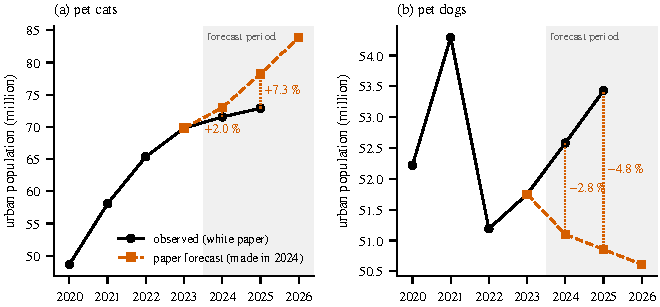
\includegraphics[width=0.72\textwidth]{figE1_forecast_vs_observed.pdf}
\caption{The paper's forecasts (Section 5, combined model) against the observed urban cat and dog populations (White Paper editions of 2020, 2025 and 2026).}\label{fig:pet-e1}
\end{figure}

The one-year-ahead errors are small, $+2.0$\,\% for cats and $-2.8$\,\% for dogs, and on their own they would suggest a successful forecast. The second year shows what the models actually learned (Figure~\ref{fig:pet-e1}). The trend models extrapolated the regime of 2019--2023, in which cats grew quickly and dogs declined slowly, whereas both populations then entered a common phase of low growth of about 2\,\% a year. The cat error therefore compounds, from $+2.0$\,\% to $+7.3$\,\% in one year, and the forecast growth of 7.2\,\% in 2025 compares with an observed 1.9\,\%. For dogs the level error is moderate, but the direction is wrong: the paper forecasts a decline and the population grew by 1.6\,\% in each year. An extrapolation of five points cannot anticipate a change of regime; a specification with saturation, such as a logistic curve or a penetration-rate model driven by household formation, would be the natural next step. The more general lesson concerns the form of the forecast. A point forecast with a stated growth rate conveys a precision that five observations cannot support, and the following section quantifies how wide an honest interval is.

\section{How much can five annual observations tell?}

\subsection{Design}
One series per species cannot show whether the miss in E1 was bad luck or a property of the method. E2 therefore evaluates the paper's method family, together with standard benchmarks, on a reference class of real annual series: the 1\,088 annual series of the \emph{Demographic} category of the M4 forecasting competition\cite{m4}. From each series one window is taken at its end, with five training values as in the paper and the next three years as targets ($h=1,2,3$); one window per series keeps the evaluation units independent. The methods are fitted to the training values only. They are the naive forecast (last value), a random walk with drift, the linear trend in time (the paper's regression), compound growth from the first to the last value (the paper's average growth rate), the grey model GM(1,1)\cite{deng1982}, an ARIMA model chosen by AIC among ARIMA(0,1,0) with and without drift, ARIMA(1,1,0) and ARIMA(0,1,1), the Theta method\cite{theta}, the paper's combination of the linear trend, GM(1,1) and ARIMA with weights inversely proportional to in-sample mean squared error, and the equal-weight combination of the same three models.

Prediction intervals are calibrated on the class in the manner of split conformal prediction\cite{lei2018}. For every method and horizon, the empirical quantiles of $\log(\text{actual}/\text{forecast})$ are estimated on a random half of the series, and the coverage of the resulting interval $[\hat y\,e^{q_{\text{lo}}},\,\hat y\,e^{q_{\text{hi}}}]$ is measured on the other half. The assumption is that windows are exchangeable within the class. The classical OLS prediction interval of the linear trend, with a $t$ distribution on three degrees of freedom, is the model-based comparator.

\subsection{Accuracy}

\begin{table}[htbp]\centering\small
\caption{Accuracy on the 1\,088 M4 Demographic windows with five training values: median absolute percentage error (\%) by horizon and the share of windows in which the method beats the naive forecast at $h=3$.}\label{tab:pet-e2}
\begin{tabular}{lcccc}\toprule
Method & $h=1$ & $h=2$ & $h=3$ & Beats naive at $h=3$\\\midrule
Naive (last value) & 2.5 & 4.6 & 6.4 & ---\\
Random walk with drift & 2.2 & 3.8 & 5.3 & 56\,\%\\
Linear trend (paper's regression) & 2.9 & 4.4 & 5.8 & 53\,\%\\
Compound growth rate (paper's CAGR) & 2.2 & 3.8 & 5.2 & 55\,\%\\
Grey model GM(1,1) & 2.5 & 3.9 & 5.4 & 55\,\%\\
ARIMA, AIC-selected & 2.2 & 3.8 & 4.8 & 38\,\%\\
Theta & 2.2 & 3.9 & 5.1 & 60\,\%\\
Inverse-MSE combination (paper's weighting) & 2.4 & 3.9 & 5.2 & 56\,\%\\
Equal-weight combination of the same three & 2.4 & 3.8 & 5.1 & 56\,\%\\\bottomrule
\end{tabular}
\end{table}

The linear trend is the least accurate of the trended methods at every horizon (Table~\ref{tab:pet-e2}); at $h=1$ it is also less accurate than the naive forecast. ARIMA has the lowest median error at $h=3$, but it beats the naive forecast in only 38\,\% of windows because its AIC selection frequently returns the random walk, in which case the two forecasts coincide. The paper's inverse-MSE weighting does not improve on equal weights, and it assigns on average the largest weight, 0.55, to the grey model: its in-sample fit is the closest of the three, but its extrapolation is no better than compound growth. The in-sample fit of the linear trend is only a weak guide to its out-of-sample error: across windows the Spearman correlation between the $R^2$ of the five-point fit and the absolute three-year error is $-0.27$. The median three-year error falls from 8.0\,\% for windows with $R^2\le 0.5$ to 4.3--4.5\,\% for $0.9<R^2\le0.99$, and only the nearly exactly linear windows ($R^2>0.99$) reach 1.4\,\%. A high $R^2$ on five points, which a steadily growing series readily produces, therefore says little about the next three years. The ordering is not specific to demographic series: on a random sample of 4\,000 of the 23\,000 annual M4 series of all categories, the linear trend is again the least accurate trended method at every horizon, with a median three-year error of 8.1\,\% against 7.4\,\% for the drift model.

\subsection{Interval calibration and direction of change}

\begin{table}[htbp]\centering\small
\caption{Empirical coverage of linear-trend prediction intervals on held-out M4 Demographic windows (five training values).}\label{tab:pet-e3}
\begin{tabular}{lcccccc}\toprule
 & \multicolumn{3}{c}{Nominal 80\,\%} & \multicolumn{3}{c}{Nominal 95\,\%}\\\cmidrule(lr){2-4}\cmidrule(lr){5-7}
Interval & $h=1$ & $h=2$ & $h=3$ & $h=1$ & $h=2$ & $h=3$\\\midrule
Classical OLS & 66\,\% & 53\,\% & 47\,\% & 87\,\% & 78\,\% & 72\,\%\\
Class-calibrated & 79\,\% & 78\,\% & 78\,\% & 96\,\% & 96\,\% & 93\,\%\\\bottomrule
\end{tabular}
\end{table}

Classical regression intervals are far too narrow for five points (Table~\ref{tab:pet-e3}). The OLS interval assumes that the linear model is correct and that its residuals are independent; with five observations the residual variance is estimated from three degrees of freedom, and the real risk, a change of slope, is outside the model altogether. Its coverage therefore falls with the horizon, to 47\,\% at nominal 80\,\% and 72\,\% at nominal 95\,\% three years ahead. The class-calibrated intervals reach 78--79\,\% and 93--96\,\%, close to nominal. Honest intervals are wide: estimated on the whole class, the calibrated 95\,\% interval of a three-year linear-trend forecast extends from $-33$\,\% to $+50$\,\% of the point forecast. The direction of a two-year change is also uncertain. The trended methods predict its sign correctly in only 63--69\,\% of windows, and the linear trend in 65\,\%.

\subsection{China from the paper's 2023 vantage point}

The class-calibrated intervals can be applied to China's series from the information set of the paper, that is, with 2019--2023 as training data. The observed values of 2024 and 2025 fall inside the calibrated 95\,\% interval of every method. For cats they fall below the 80\,\% interval of every trended method except the damped Theta method: the linear trend forecasts 84.4 million for 2025 with an 80\,\% interval of 76.5--95.1 million, and 72.9 million were observed. The cat slowdown therefore lies below the 10\,\% quantile of the class's forecast errors but above its 2.5\,\% quantile, which makes it unusual relative to the class but not implausible. The dog observations stay inside all 80\,\% intervals.

A re-implementation of the paper's combination, with the linear trend, GM(1,1) and ARIMA weighted by inverse in-sample MSE, reproduces the dog forecast closely (51.05 against 51.10 million for 2024, and 50.20 against 50.61 million for 2026). It does not reproduce the cat forecast (78.0 against 73.0 million for 2024). Because the original code was not preserved, the source of the cat discrepancy cannot be traced, and E1 evaluates the forecasts as printed in the paper.

\subsection{An updated outlook from 2025}

With seven annual values (2019--2025), ARIMA is the most accurate method of the class at $h=1$ and $h=3$, and within 0.02 percentage points of compound growth at $h=2$. Table~\ref{tab:pet-e4} gives its forecasts with class-calibrated intervals estimated on seven-value windows.

\begin{table}[htbp]\centering\small
\caption{Outlook from 2025: ARIMA forecasts with class-calibrated 80\,\% and 95\,\% intervals (urban China, $10^4$ animals).}\label{tab:pet-e4}
\begin{tabular}{lrccrcc}\toprule
 & 2026 & 80\,\% & 95\,\% & 2028 & 80\,\% & 95\,\%\\\midrule
Urban cats & 7\,393 & 6\,980--7\,903 & 6\,023--9\,081 & 7\,533 & 6\,785--8\,725 & 5\,209--10\,739\\
Urban dogs & 5\,284 & 4\,989--5\,649 & 4\,305--6\,490 & 5\,297 & 4\,771--6\,135 & 3\,663--7\,551\\\bottomrule
\end{tabular}
\end{table}

\begin{figure}[htbp]\centering
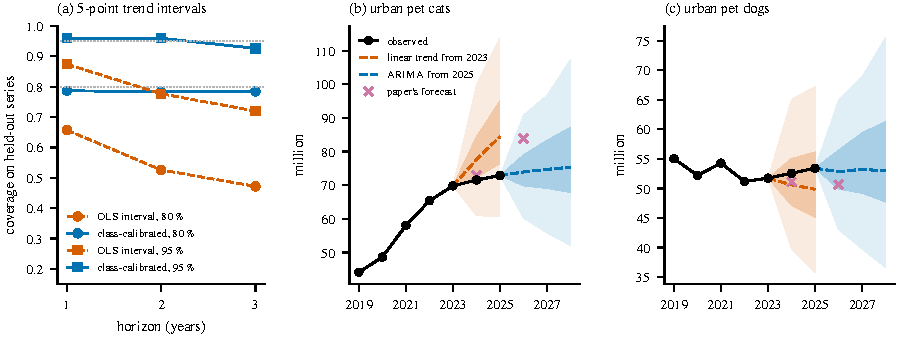
\includegraphics[width=\textwidth]{figE2_reference_class.pdf}
\caption{(a) Coverage of nominal 80\,\% (circles) and 95\,\% (squares) intervals for five-point linear-trend forecasts on held-out M4 Demographic series: classical OLS intervals against class-calibrated intervals. (b, c) Observed series, the linear-trend forecast from 2023 with calibrated bands for the two check years, the ARIMA outlook from 2025, and the paper's forecasts.}\label{fig:pet-e2}
\end{figure}

The trended alternatives put cats higher in 2026: the Theta method forecasts 75.46 million, the drift model 77.69 million and the linear trend 82.04 million. This spread, about 8 million animals between ARIMA and the linear trend, is itself the main result (Figure~\ref{fig:pet-e2}). With seven annual points the defensible statement about 2026 is an interval of roughly 70--79 million cats at 80\,\% confidence, not a growth rate.

\subsection{Conclusions and limits}

The forecasting layer of the paper was accurate one year ahead and then drifted away in the way that the reference class shows to be typical of five-point trend extrapolation: it projected a regime that ended. The class evaluation shows that the paper's choice of the linear trend and of inverse-MSE weighting did not help, and that the precision implied by point forecasts and classical regression intervals was overstated, since those intervals cover the outcome three years ahead in fewer than three cases out of four at a nominal 95\,\%. Since the demand and industry models of Problems 2--4 take these forecasts as inputs, their outputs inherit the same uncertainty; propagating the calibrated intervals through those models would be the consistent next step, but their inputs were not preserved with the entry and they are not re-estimated here. The reference class is a judgement. M4 demographic series are statistics of human populations rather than of pet populations, and the calibrated intervals are valid only to the extent that China's pet series behave like a draw from that class. The results for 2024--2025 are consistent with this assumption, since both species fall inside the calibrated 95\,\% intervals, but two years of two series cannot confirm it.

\begin{thebibliography}{9}
\bibitem{petdata} Petdata ({\cjkfont 派读宠物行业大数据平台}). \emph{China Pet Industry White Paper} ({\cjkfont 中国宠物行业白皮书}), consumer reports, 2020, 2025 and 2026 editions.
\bibitem{m4} S. Makridakis, E. Spiliotis, V. Assimakopoulos. The M4 Competition: 100,000 time series and 61 forecasting methods. \emph{International Journal of Forecasting}, 36(1): 54--74, 2020. doi:10.1016/j.ijforecast.2019.04.014.
\bibitem{deng1982} J.-L. Deng. Control problems of grey systems. \emph{Systems \& Control Letters}, 1(5): 288--294, 1982. doi:10.1016/S0167-6911(82)80025-X.
\bibitem{theta} V. Assimakopoulos, K. Nikolopoulos. The theta model: a decomposition approach to forecasting. \emph{International Journal of Forecasting}, 16(4): 521--530, 2000. doi:10.1016/S0169-2070(00)00066-2.
\bibitem{lei2018} J. Lei, M. G'Sell, A. Rinaldo, R. J. Tibshirani, L. Wasserman. Distribution-free predictive inference for regression. \emph{Journal of the American Statistical Association}, 113(523): 1094--1111, 2018. doi:10.1080/01621459.2017.1307116.
\end{thebibliography}
\end{document}
